%\documentclass[letterpaper,10pt,oneside,conference,final]{sbrt2015}
\documentclass{sbrt2015}
%\documentclass{sbrt2015}

\usepackage{enumerate} 

\begin{document}
  \IEEEoverridecommandlockouts

  \title{On the Stability of Delay-Centric Multihomed Transmission}
  \author
  {
    \authorblockN{Pedro Mantovani Antunes, Guilherme de Souza Miguel,\\
                  Carlos Marcelo Pedroso, Eduardo Parente Ribeiro\\}
    \authorblockA{Federal University of Parana - UFPR\\
                  P.O. Box 19011 -- 81531-980\\
                  Curitiba -- PR -- Brazil\\
                  edu@ufpr.br}
  }
  \maketitle
  
  
%  \markboth{XXXIII SIMPOSIO BRASILEIRO DE TELECOMUNICACOES - SBrT2015, 1-4 DE SETEMBRO DE 2015, JUIZ DE FORA, MG} {XXXIII SIMPOSIO BRASILEIRO DE TELECOMUNICACOES - SBrT2015, 1-4 DE SETEMBRO DE 2015, JUIZ DE FORA, MG}

  \begin{abstract}
    The use of multiple network interfaces for multimedia transmission can reduce packet delay by choosing the less congested end-to-end path for transmission. Delay-centric is a simple mechanism that selects the path with current lowest delay. When multiple users employ this mechanism there is a possibility of instabilities due to excessive path changes that increases overall packet delay. In this paper we investigate some modifications on the delay-centric algorithm to reduce overall transmission latency in a scenario with multiple independent transmissions.
  \end{abstract}

  \begin{keywords}
    multihome, end-to-end multipath, delay-centric, SCTP.
  \end{keywords}


  \section{Introduction}

  Multihoming has been gaining increasing popularity in the recent years. Users can be connected to the Internet by different network access technologies such as ADSL (Asymmetric Digital Subscriber Line), Wi-Fi, WiMaX (Worldwide Interoperability for Microwave Access), 3G and LTE (Long Term Evolution). Multimedia communication can benefit from multiple end-to-end paths by selecting the best available path for transmission at a particular time, thus avoiding congestion and reducing packet loss.

A framework for multihomed communication was established by the Stream Control Transmission Protocol (SCTP) \cite{Stewart2007a}, but other approaches are possible, such as Multipath Transmission Control Protocol (MPTCP) \cite{Ford2013}\cite{Zekri2012} and application layer handover \cite{Cunningham2004}. The standard SCTP protocol monitors the availability of each end-to-end path and automatically switches transmission to a secondary path in case of failure in the primary path to increase resilience. Other utilizations of multihoming already proposed in the literature include concurrent multipath transfer (CMT) \cite{Casetti2004}\cite{Ye2004}\cite{Iyengar2006}, seamless handoff for mobile users \cite{Koh2004}\cite{Ma2004} and delay-centric transmission for low-delay communication \cite{Kelly2004}\cite{Kashihara2004}. The latter is suitable for real-time multimedia transmissions.
The benefits of the delay-centric algorithm for a single multimedia transmission have already been shown by several authors \cite{Noonan2004b}\cite{Fitzpatrick2007}\cite{Gavriloff2009a}\cite{Runcos2010}. 

One topic that has not been fully investigated is the stability issue that arises when multiple users employ the delay-centric mechanism. An initial investigation has shown that under high link utilization, overall packet delay can increase due to excess of path changes of the transmitting sources \cite{Gavriloff2009}.
In this paper, we investigate some preventing measures that can be taken to mitigate these instabilities and to allow lower end-to-end delay for all users.

The remainder of this paper is divided into four sections. Section II describes some fundamentals of delay-centric SCTP transmission. Section III explains the implemented methods. Results are shown in Section IV e conclusion is presented in Section V.  

  \section{Multihomed low-delay communication}
  
  \subsection{Latency Estimation}

  Latency estimation of the end-to-end path is performed in both SCTP and TCP to calculate the retransmission timeout (RTO) of each packet \cite{Stewart2007a}\cite{Postel1981}. To achieve this estimation, these protocols measure the round trip time (RTT) of a packet every time an acknowledge is received. As this value is highly variable, the protocol uses the smoothed round trip time (SRTT), defined as
\begin{equation}
SRTT_i  = (1 - \alpha) SRTT_{i-1} + \alpha  RTT \\
\end{equation}
\noindent where $\alpha$ value is 0.125, as recommended by RFC 4960 \cite{Stewart2007a} and RFC 6298 \cite{Paxson2011}.


  \subsection{Delay-centric}

  Delay-centric method compares the SRTT of all paths to decide where to transmit the packets \cite{Kelly2004}. The SRTT of the primary path is updated frequently, because it is changed every time an ACK of a transmitted packet is received. In the secondary paths, the SRTT is updated only after a heartbeat-ack (HB-ACK) of a sent heartbeat (HB) is received. This does not give these paths a proper estimation of its latency, as the standard interval between HBs is 30\,s. To improve the algorithm's responsiveness, most authors employed the value of 1\,s for the HB interval \cite{Noonan2004b}\cite{Gavriloff2009}\cite{Torres2014}.

The path handover in delay-centric method occurs when the difference between the SRTT of the current path and the SRTT of an alternate path becomes greater than zero, or greater than a threshold, called hysteresis.

A variation of the delay-centric method includes the utilization of a guard-time \cite{Leung2012}. This is the period to wait after the SRTT comparison indicated a path handover. At the end of this period, the SRTTs are compared again, to check if the current SRTT is still greater than the SRTT of the alternate path, to confirm the handover or to cancel it, and keep the transmission in the same path. A random value is selected for each new period to prevent synchronous operation of the sources and to promote better distribution of the handover decision over the time. In this paper, we propose the reduction of the heartbeat interval to 20\,ms during guard-time, in order to improve the estimate of the delay over the alternate path.

  \subsection{Predictive delay-centric}

  A recent improvement in the delay-centric method also considers the SRTT trend \cite{Torres2014}. The moving average convergence divergence (MACD) method is used. For each path, two SRTTs are calculated. A short time version, with $\alpha = 0.667$, named $SRTT_S$, and a long time version with $\alpha = 0.154$, named $SRTT_L$. When the $SRTT_S$ becomes greater than $SRTT_L$, there is a trend to increase latency. The handover algorithm takes this trend into account and performs the handover only when these three conditions hold:
\begin{enumerate}[i)]
 \item Current path SRTT is increasing ($SRTT_S > SRTT_L$).
 \item $SRTT_S$ of current path is greater than a threshold, set at 150\,ms.
 \item $SRTT_S$ of current path greater than $SRTT_S$ of alternate path.
\end{enumerate}

Simulations with typical delays gathered from Wi-Fi, 3G and Ethernet, have shown that this strategy, called predictive delay-centric (PDC), improves the quality of video transmission and reduces the number of handovers compared to pure delay-centric, which is a reactive method (RDC).

In this paper, we use a modified version of predictive delay-centric. We replace condition (i) by:
${(SRTT_S - SRTT_L) > (srtt_S - srtt_L)}$, where upper case SRTT is the SRTT of the primary path, while the lower case is the SRTT of the alternate path. This condition is an indication that the trend of increasing latency is greater in the current path than it is in the alternate path. This change requires the calculation of SRTT trend on both primary and secondary paths. Switchover will occur if the alternate path has more favorable conditions in terms of latency trend than the primary path, and if conditions (ii) and (iii) are also true. 

\section{Methods}

The test bed consisted of two computers connected to each other by two Ethernet links, as illustrated in Figure~\ref{topology}. In our last simulation, the same methodology was applied to check the algorithms' behavior in the presence of a third Ethernet link.

\begin{figure}[ht!]
\centering
%\includegraphics[width=8.5cm]{figuras/cadeiamark.ps}
%\includegraphics[scale=0.3]{gilbert}
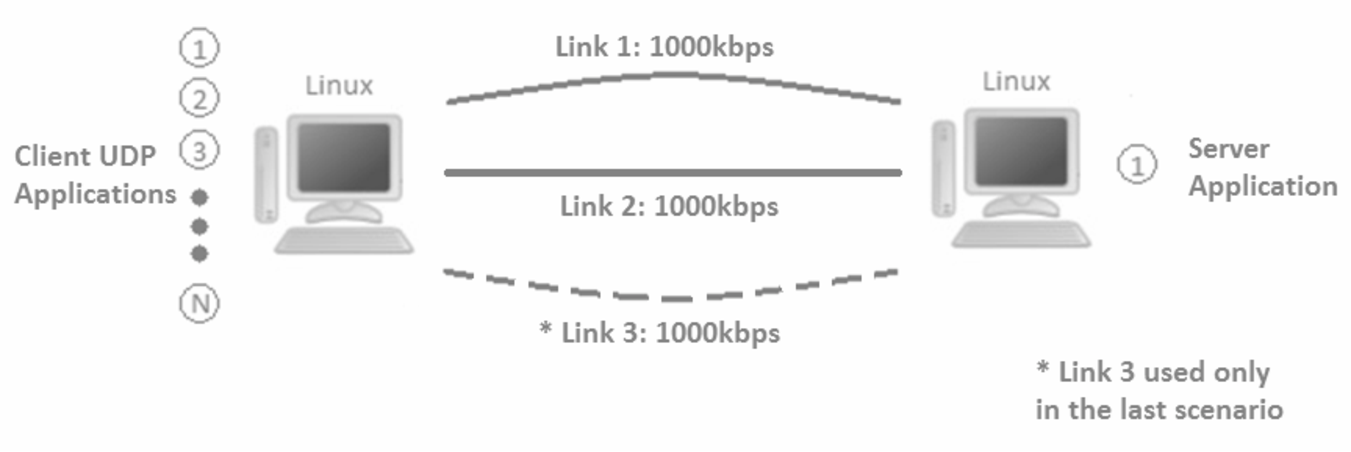
\includegraphics[width=8.8cm,height=3cm]{figura1}
\caption{Topology used in the experiments.}
\label{topology}
\end{figure}

Both machines operate with Linux operating system (distribution Debian 7.1, Linux kernel 3.2.63-2). Test programs were written in C and compiled with gcc version 4.7.2-5. The multimedia transmission data consisted of 6 sources that independently transmitted UDP (User Datagram Protocol) packets with 250 bytes of size, including headers. Each source also transmits heartbeat packets of 55 bytes in the alternate path. All ACK packets have 52 bytes. Each multimedia source starts its transmission randomly during the first second of the experiment. In order to work with lower bit rates, the bandwidth of the transmission was limited with the kernel traffic control (tc). 

A total of 3000 packets were sent on each experiment, which was repeated 200 times to estimate the mean packet delay, its standard deviation and confidence intervals. In each experiment, the mean packet delay was measured for different path utilizations. The definition of path utilization was extended to consider a multipath scenario. The aggregated utilization is calculated as 

\begin{equation}
 \rho = \frac{\sum\limits_{i=1}^{t}A_i + \sum\limits_{i=1}^{n}B_i}{\sum\limits_{i=1}^{n}C_i}
\end{equation}
where \textit{t} is the number of active transmissions and \textit{A} is the transmission traffic bit rate. The number of active paths is \textit{n} and \textit{B} is the background traffic bit rate. The individual path capacity is \textit{C}. In the experiments, the number of active transmissions (\textit{t}) was 6 and the number of paths (\textit{n}) was 2, except in the last experiment that had a third path. The link capacity was 1\,Mbps for each path. 
The background traffic was zero in the initial test, but then changed to a given proportion of the total traffic in the subsequent tests. In all the simulations, $\rho$ was varied from 0.72 to 0.99 by altering the values of \textit{A} and \textit{B}.

The following mechanisms were tested:
\begin{enumerate}[i)]
 \item Pure delay-centric, hysteresis = 10\,ms.
 \item Delay-centric, hysteresis = 10\,ms, guard-time = 1 -- 4\,s (heartbeat interval during guard-time = 20\,ms).
 \item Predictive delay-centric.
 \item Predictive delay-centric, guard-time = 1 -- 4\,s (heartbeat interval during guard-time = 20\,ms).
\end{enumerate}

Heartbeat interval on all mechanisms were set to a random value between 0.5\,s and 1.5\,s generated after each heartbeat, except when in guard-time period, when it is changed to 20 ms.
Because the bandwidth was limited in the sender machine, the queue delay was originated in the sender side only. The delay on the return path was negligible. To compensate that, we adjusted handover threshold in the predictive delay-centric experiments to 70\,ms.

The mechanisms were also simulated with the presence of background traffic. The background traffic consisted of fixed size UDP packets (250 bytes) with random, exponentially distributed inter-arrival time. Different proportions of background and foreground traffic were analyzed, but in order to simplify the results, we decided to present only the proportion of 40\% background traffic against 60\% of foreground traffic, which gives a representative comparison among all mechanisms in a different scenario.

\section{Results}
\subsection{Algorithms' Behavior}
The first round of experiments was executed without any background traffic. For a particular aggregated utilization, the average delay was evaluated after 200 repetitions. The obtained histogram of empirical end-to-end delay did not exhibit a single mode, but two modes. One of them is close to zero milliseconds (minimum delay) and the other mode is between zero and the maximum delay. The interpretation of this result is that regarding some initial conditions, the mechanisms were able to distribute all flows over the available paths and achieve low delay for all flows. But other initial conditions led to non-stable behavior and the transmissions kept changing paths. This resulted in large average delays for all flows. Figure~\ref{figura2} displays the average delay as a function of the utilization. All analyzed handover methods are presented in Figure~\ref{figura2} with their respective average packet delay. For each curve, confidence intervals (95\%) are also plotted.

\begin{figure}[h!]
\centering
%\includegraphics[width=8.5cm]{figuras/cadeiamark.ps}
%\includegraphics[scale=0.3]{gilbert}
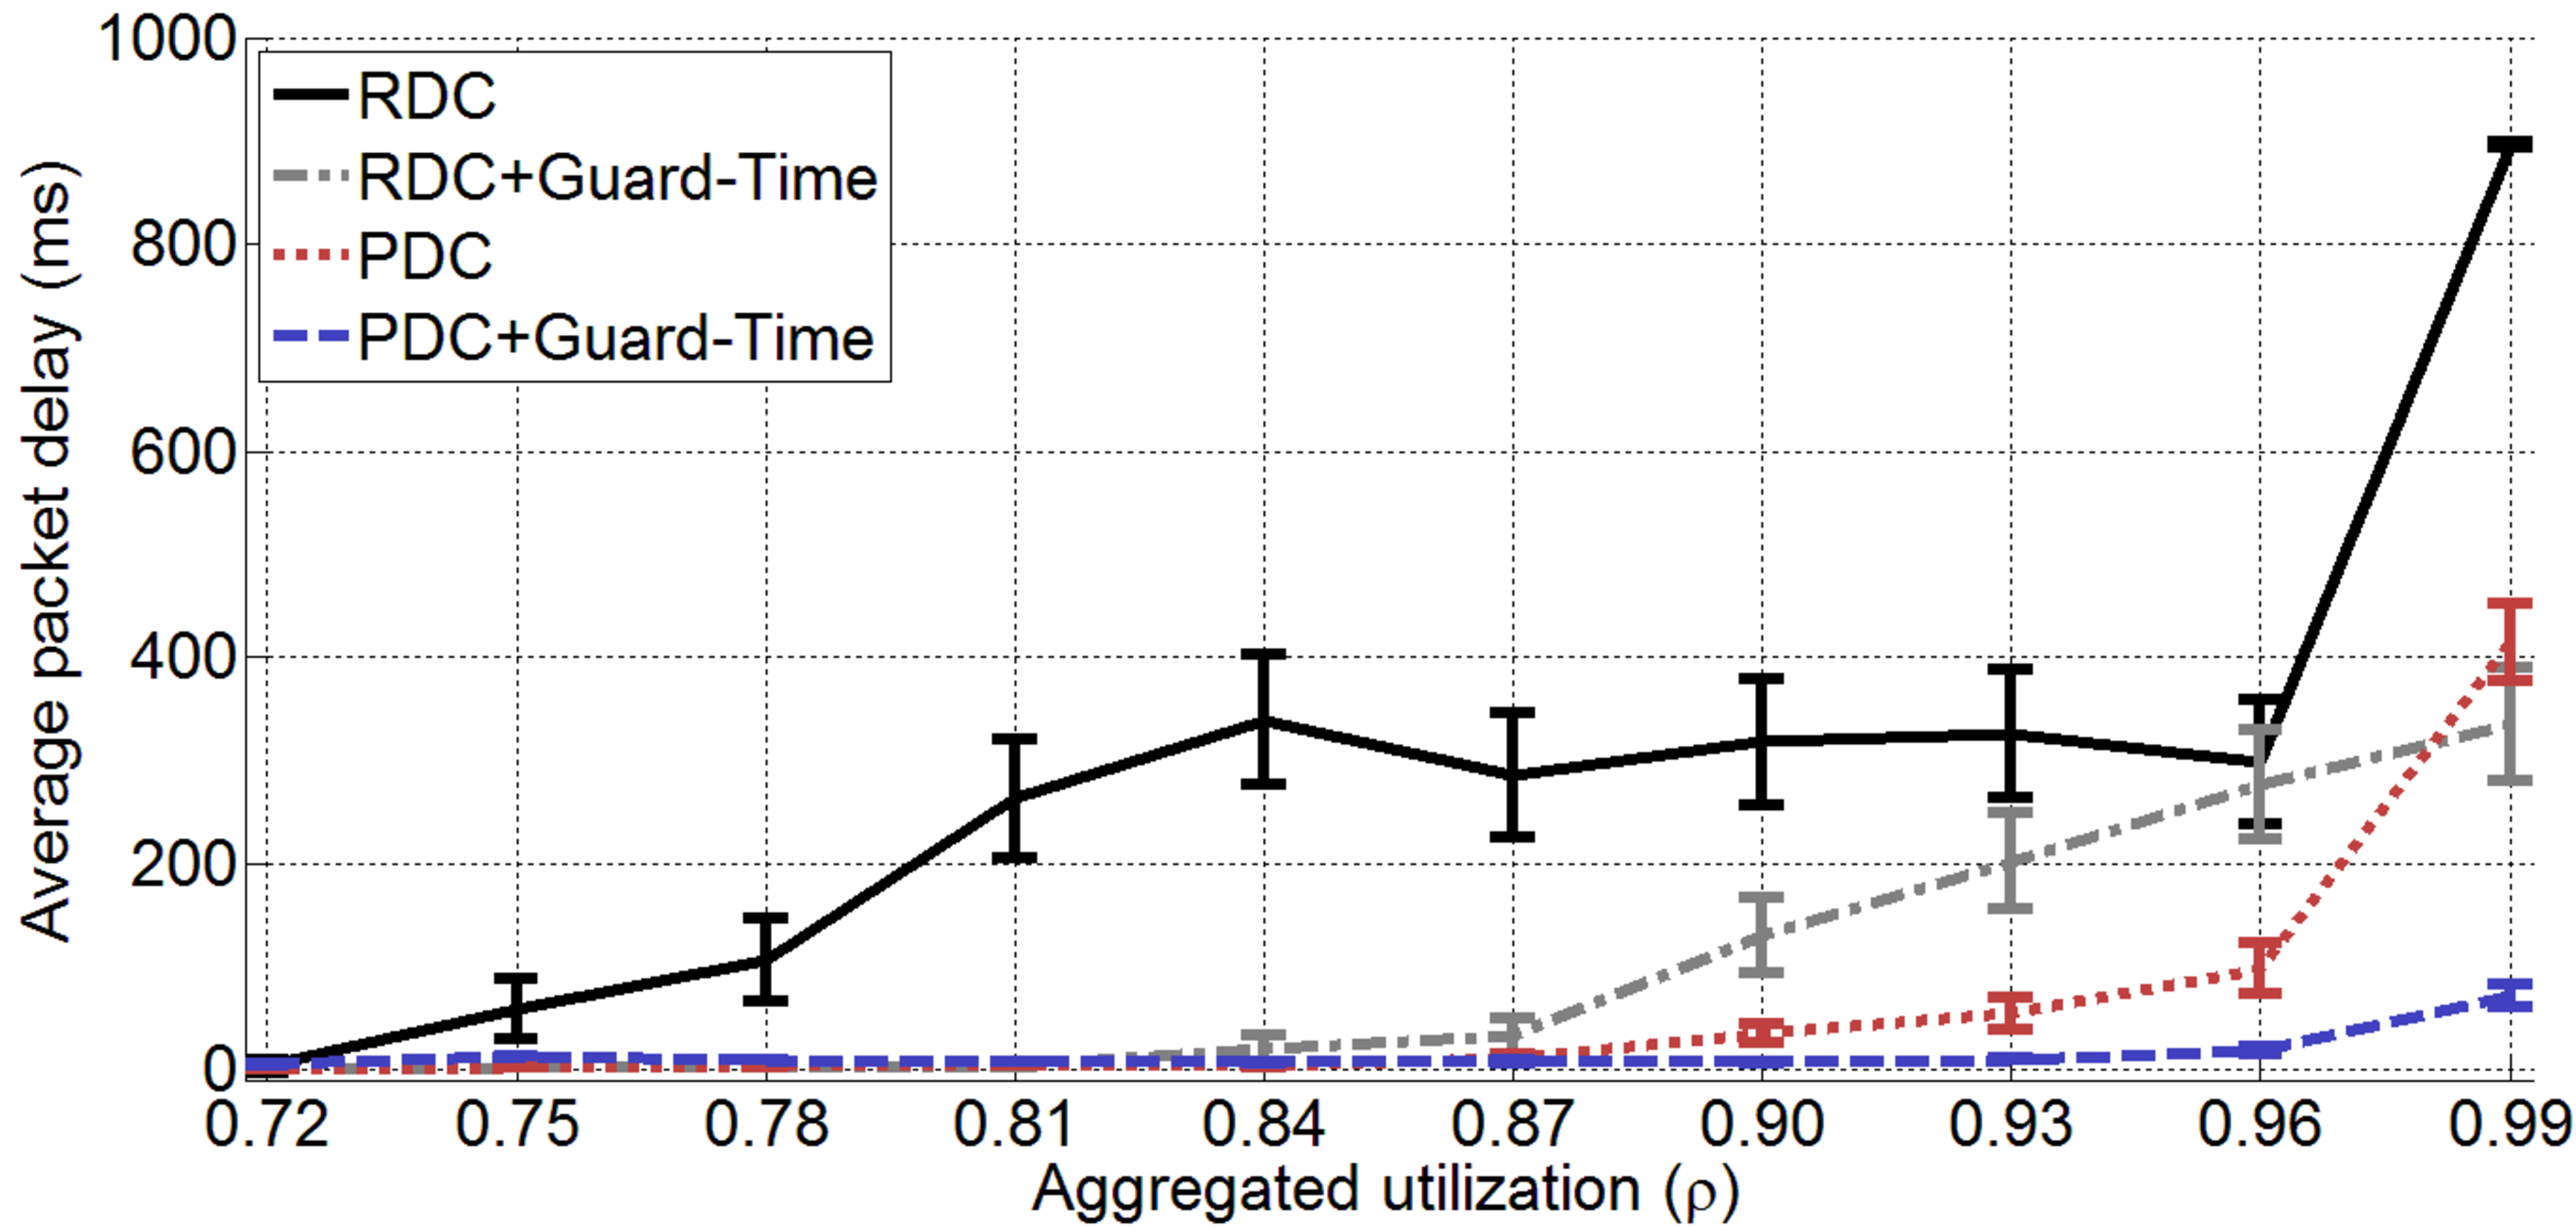
\includegraphics[width=8.8cm,height=4.5cm]{figura2}
\caption{Algorithms' behavior without background traffic.}
\label{figura2}
\end{figure}

For low utilizations ($\rho < 0.75$) the pure reactive delay-centric (RDC) mechanism was able to promote an even distribution of the transmissions over the two paths. As expected in higher utilizations ($\rho > 0.75$), instabilities may occur and the excessive path changes increase the overall mean delay. This instability problem is mainly caused by poor latency estimation of the secondary path, due to fact that the HB intervals (1\,s) are much longer than the data packet interval (approximately 20\,ms). Shortening these intervals too much may not be a good solution, since the HBs would consume unnecessary bandwidth. The reduction of HB interval during guard-time only proved to be a good compromise yielding improved latency estimation with low overhead. 
The tests in Figure~\ref{figura2} showed that RDC with guard-time resulted in lower packet delay compared to the pure RDC. It may have given the transmissions a better estimative of the SRTTs, leading to a improved handover decision.

The predictive delay-centric (PDC) method was also evaluated: both the pure predictive delay-centric, and the predictive delay-centric with guard-time and HB interval reduction. The pure PDC algorithm resulted in lower packet delay than the pure RDC, which indicates its ability to avoid instabilities by detecting the trends of SRTTs.
Following the behavior of RDC, the guard-time with HB interval reduction implemented in PDC helped to lower the overall delay even more, eliminating almost every case of instability. With this mechanism, even in high utilization ($\rho$ = 0.99), the average delay was not high enough to greatly affect the QoS (Quality of Service) of a VoIP (Voice over IP) call, for example.

\subsection{Background Traffic Scenario}
Additional experiments were conducted with background traffic to investigate the performance of the handover mechanisms in more realistic scenario. 
We noted that the addition of background traffic resulted in an unimodal distribution for all mechanisms.

Figure~\ref{figura6} presents the comparison between the handover methods. In this test, all the sources represent 60\% of the total traffic and background traffic represents 40\% of total traffic. The mean delay and confidence intervals (95\%) for each method were plotted. The predictive delay-centric with guard-time also had better stability than all the other algorithms. It was able to keep low delay for all sources of transmission, even for utilization as high as 0.99.


\begin{figure}[h!]
\centering
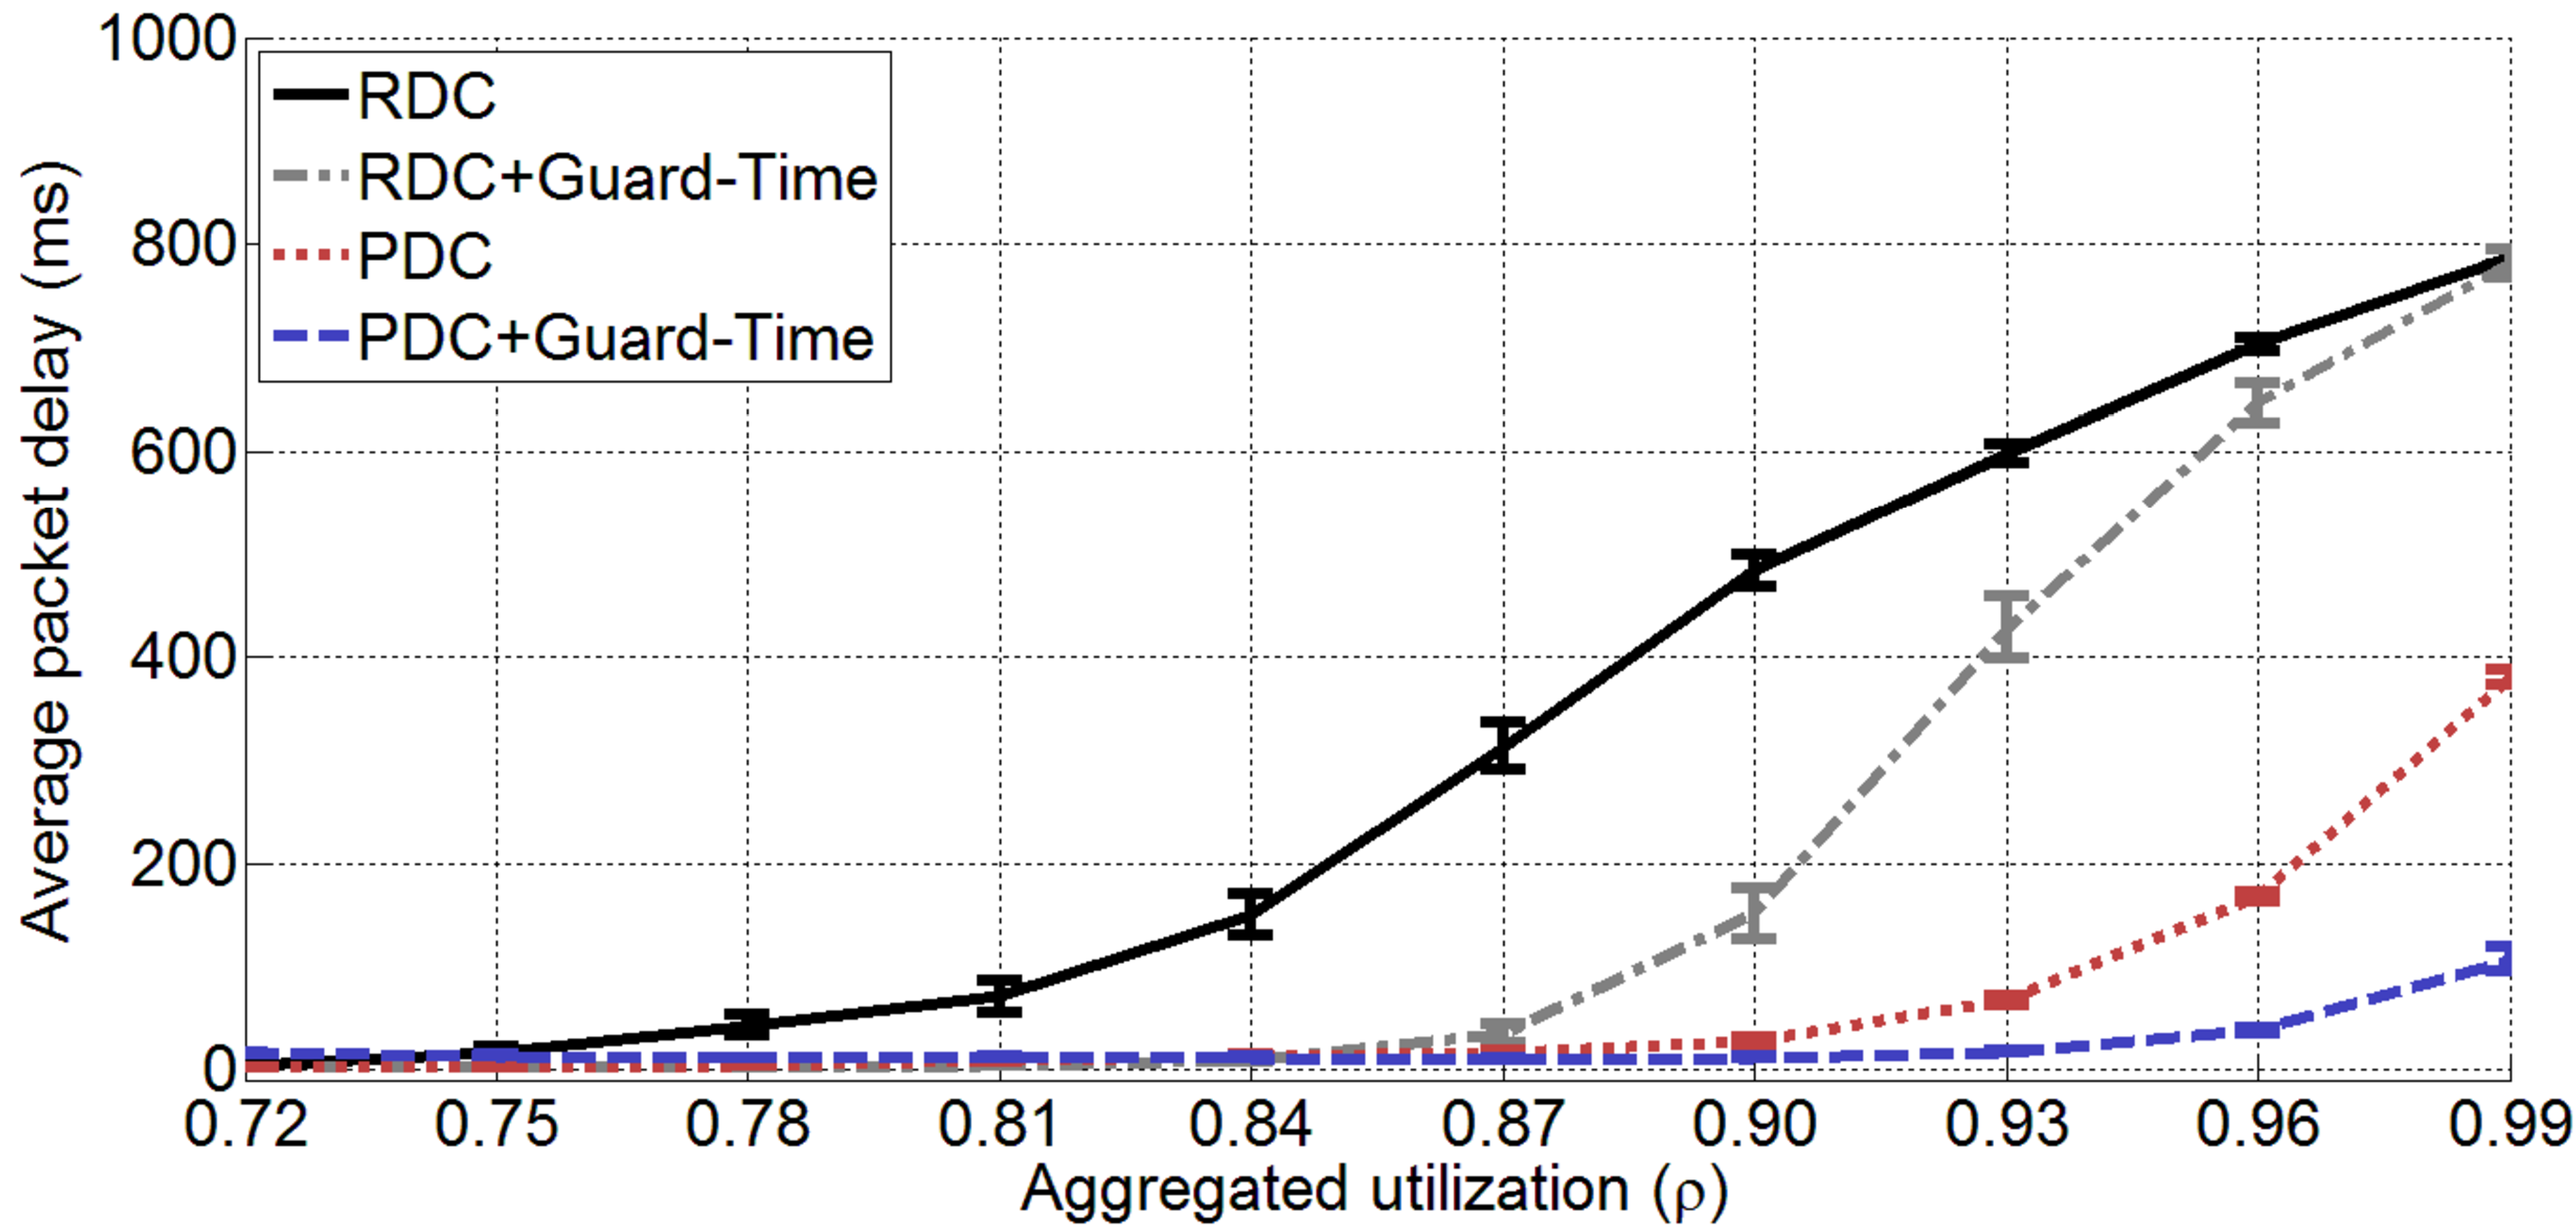
\includegraphics[width=8.8cm,height=4.3cm]{figura6}
\caption{Scenario with random background traffic.}
\label{figura6}
\end{figure}

\subsection{Comparison of Predictive delay-centric methods}
A comparison between the original PDC method and the modified PDC method was performed and results are displayed in Figure~\ref{figura7}.
Without the guard-time, the algorithms acted almost in the same way, and yielded similar mean packet delay values. 
With the guard-time implemented, the modified PDC method exhibited lower delays at higher utilization levels. 
The trend of secondary paths could now be calculated more accurately because of the decrease in the HB interval during guard-time, giving the modified algorithm
more stability. 


\begin{figure}[h!]
	\centering
	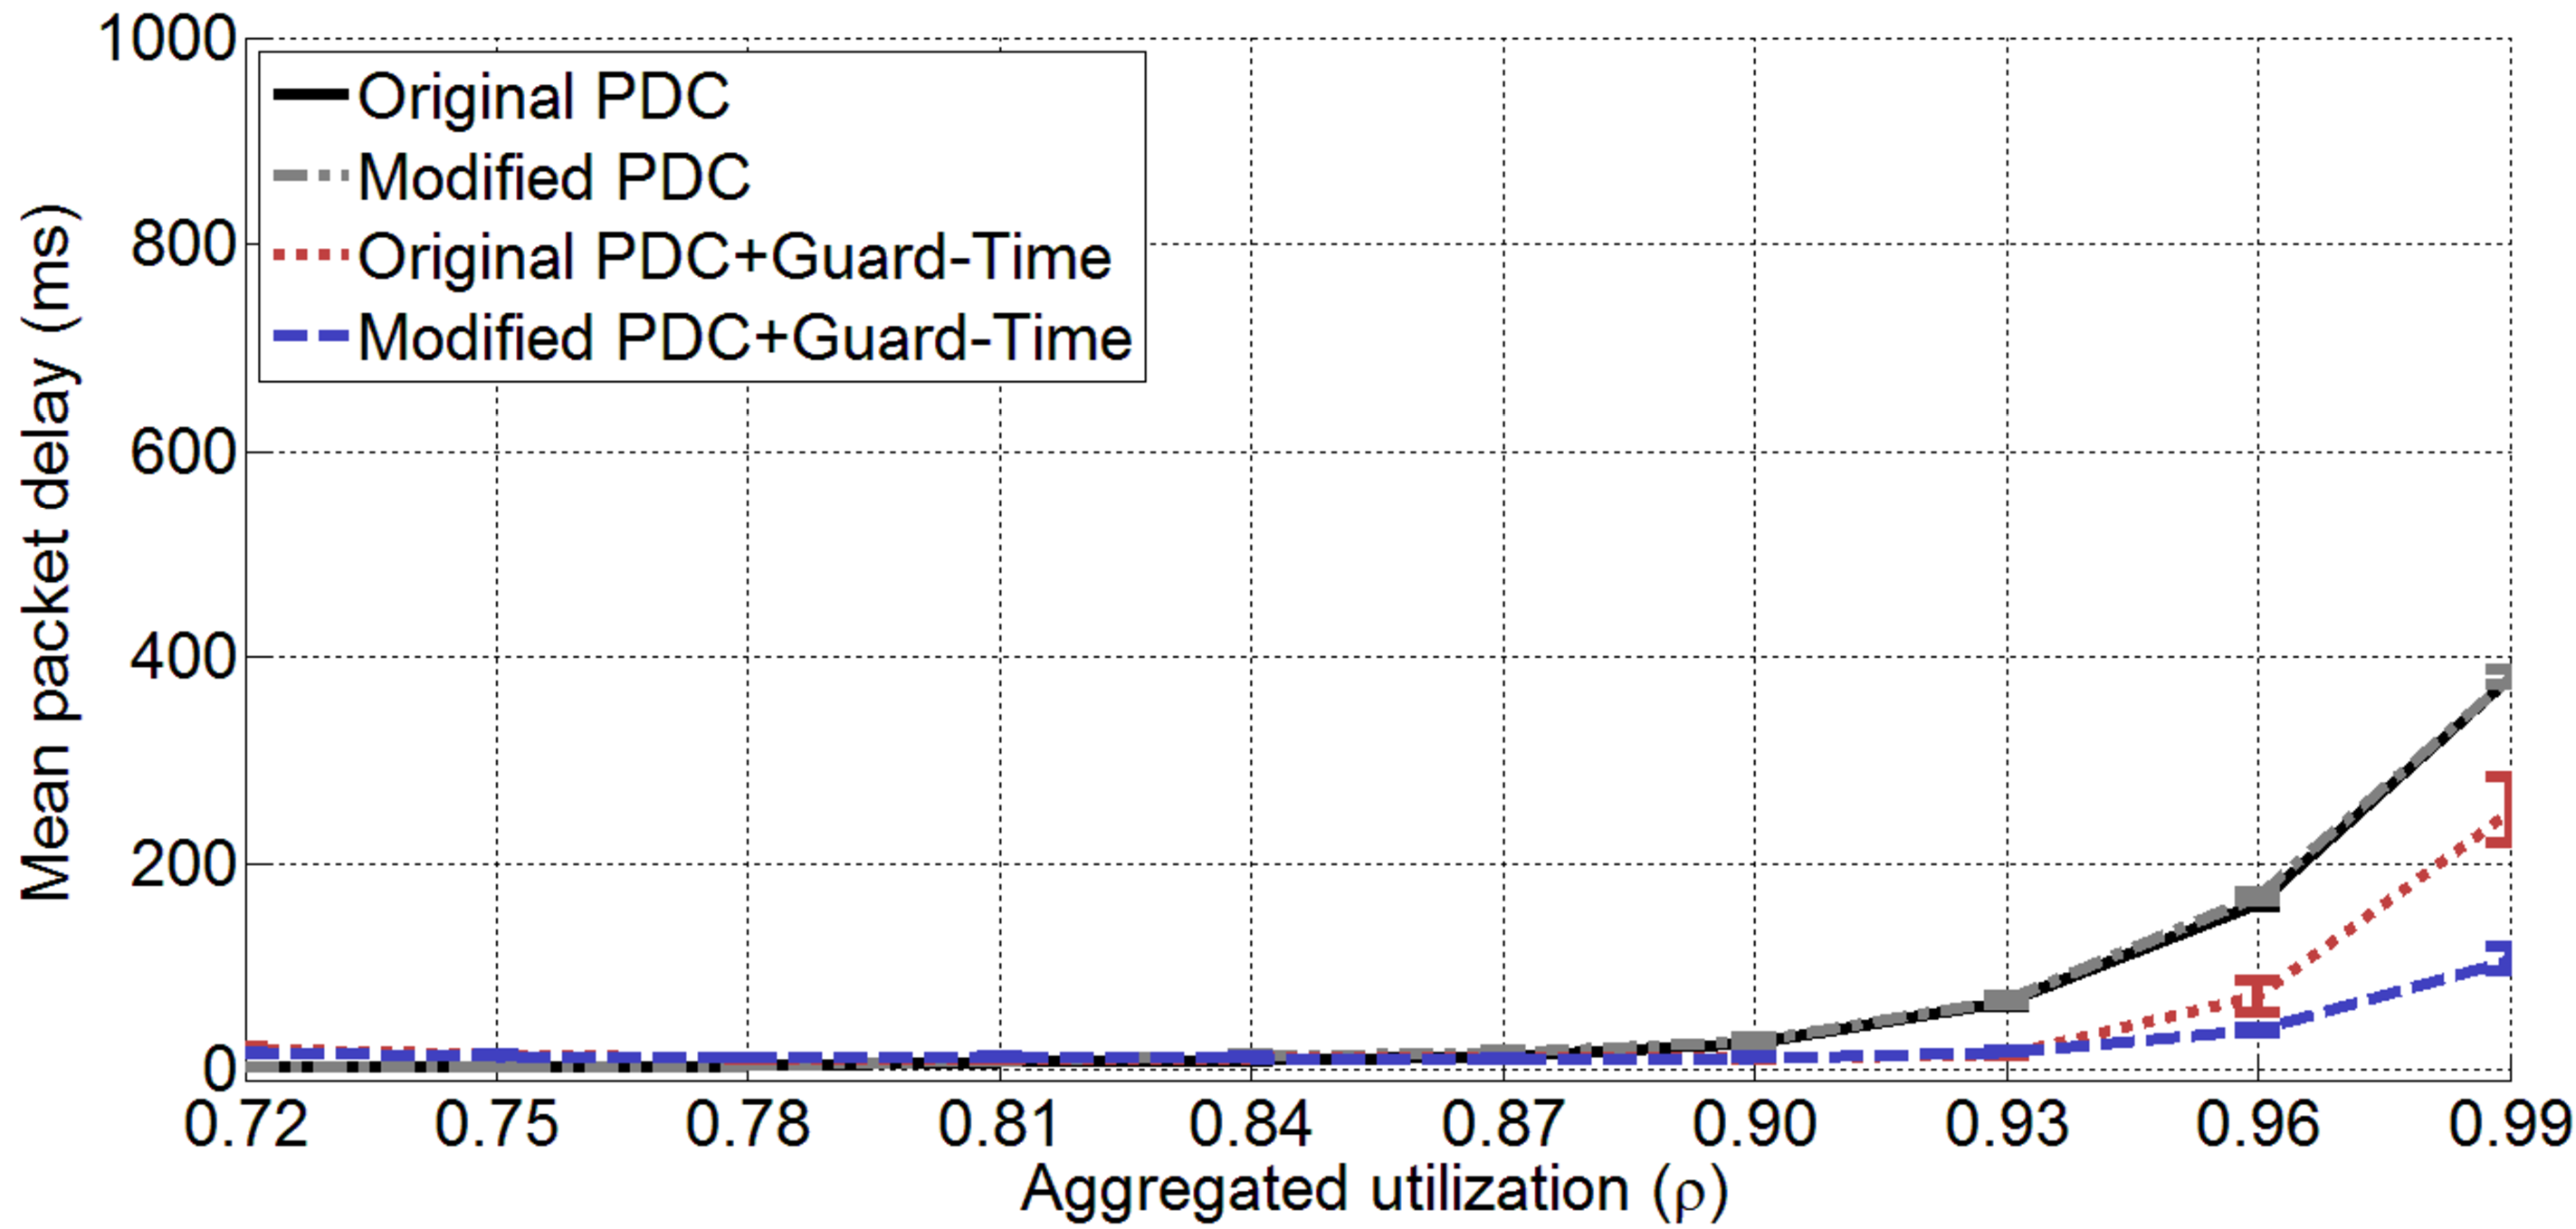
\includegraphics[width=8.8cm,height=4.3cm]{figura7}
	\caption{Comparison between predictive delay-centric methods.}
	\label{figura7}
\end{figure}

\subsection{Algorithms' Behavior with a third path}
All methods were tested with 3 paths to verify how the handover algorithm scale with the number of paths.
The proportion of background traffic was 40\% of total traffic, the same as in previous tests. 
Figure~\ref{figura8} shows the results for RDC and RDC with Guard-Time, and Figure~\ref{figura9} shows the results for PDC and PDC with Guard-Time. 
In both figures, the results obtained with 2 paths are also plotted for comparison.


\begin{figure}[h!]
	\centering
	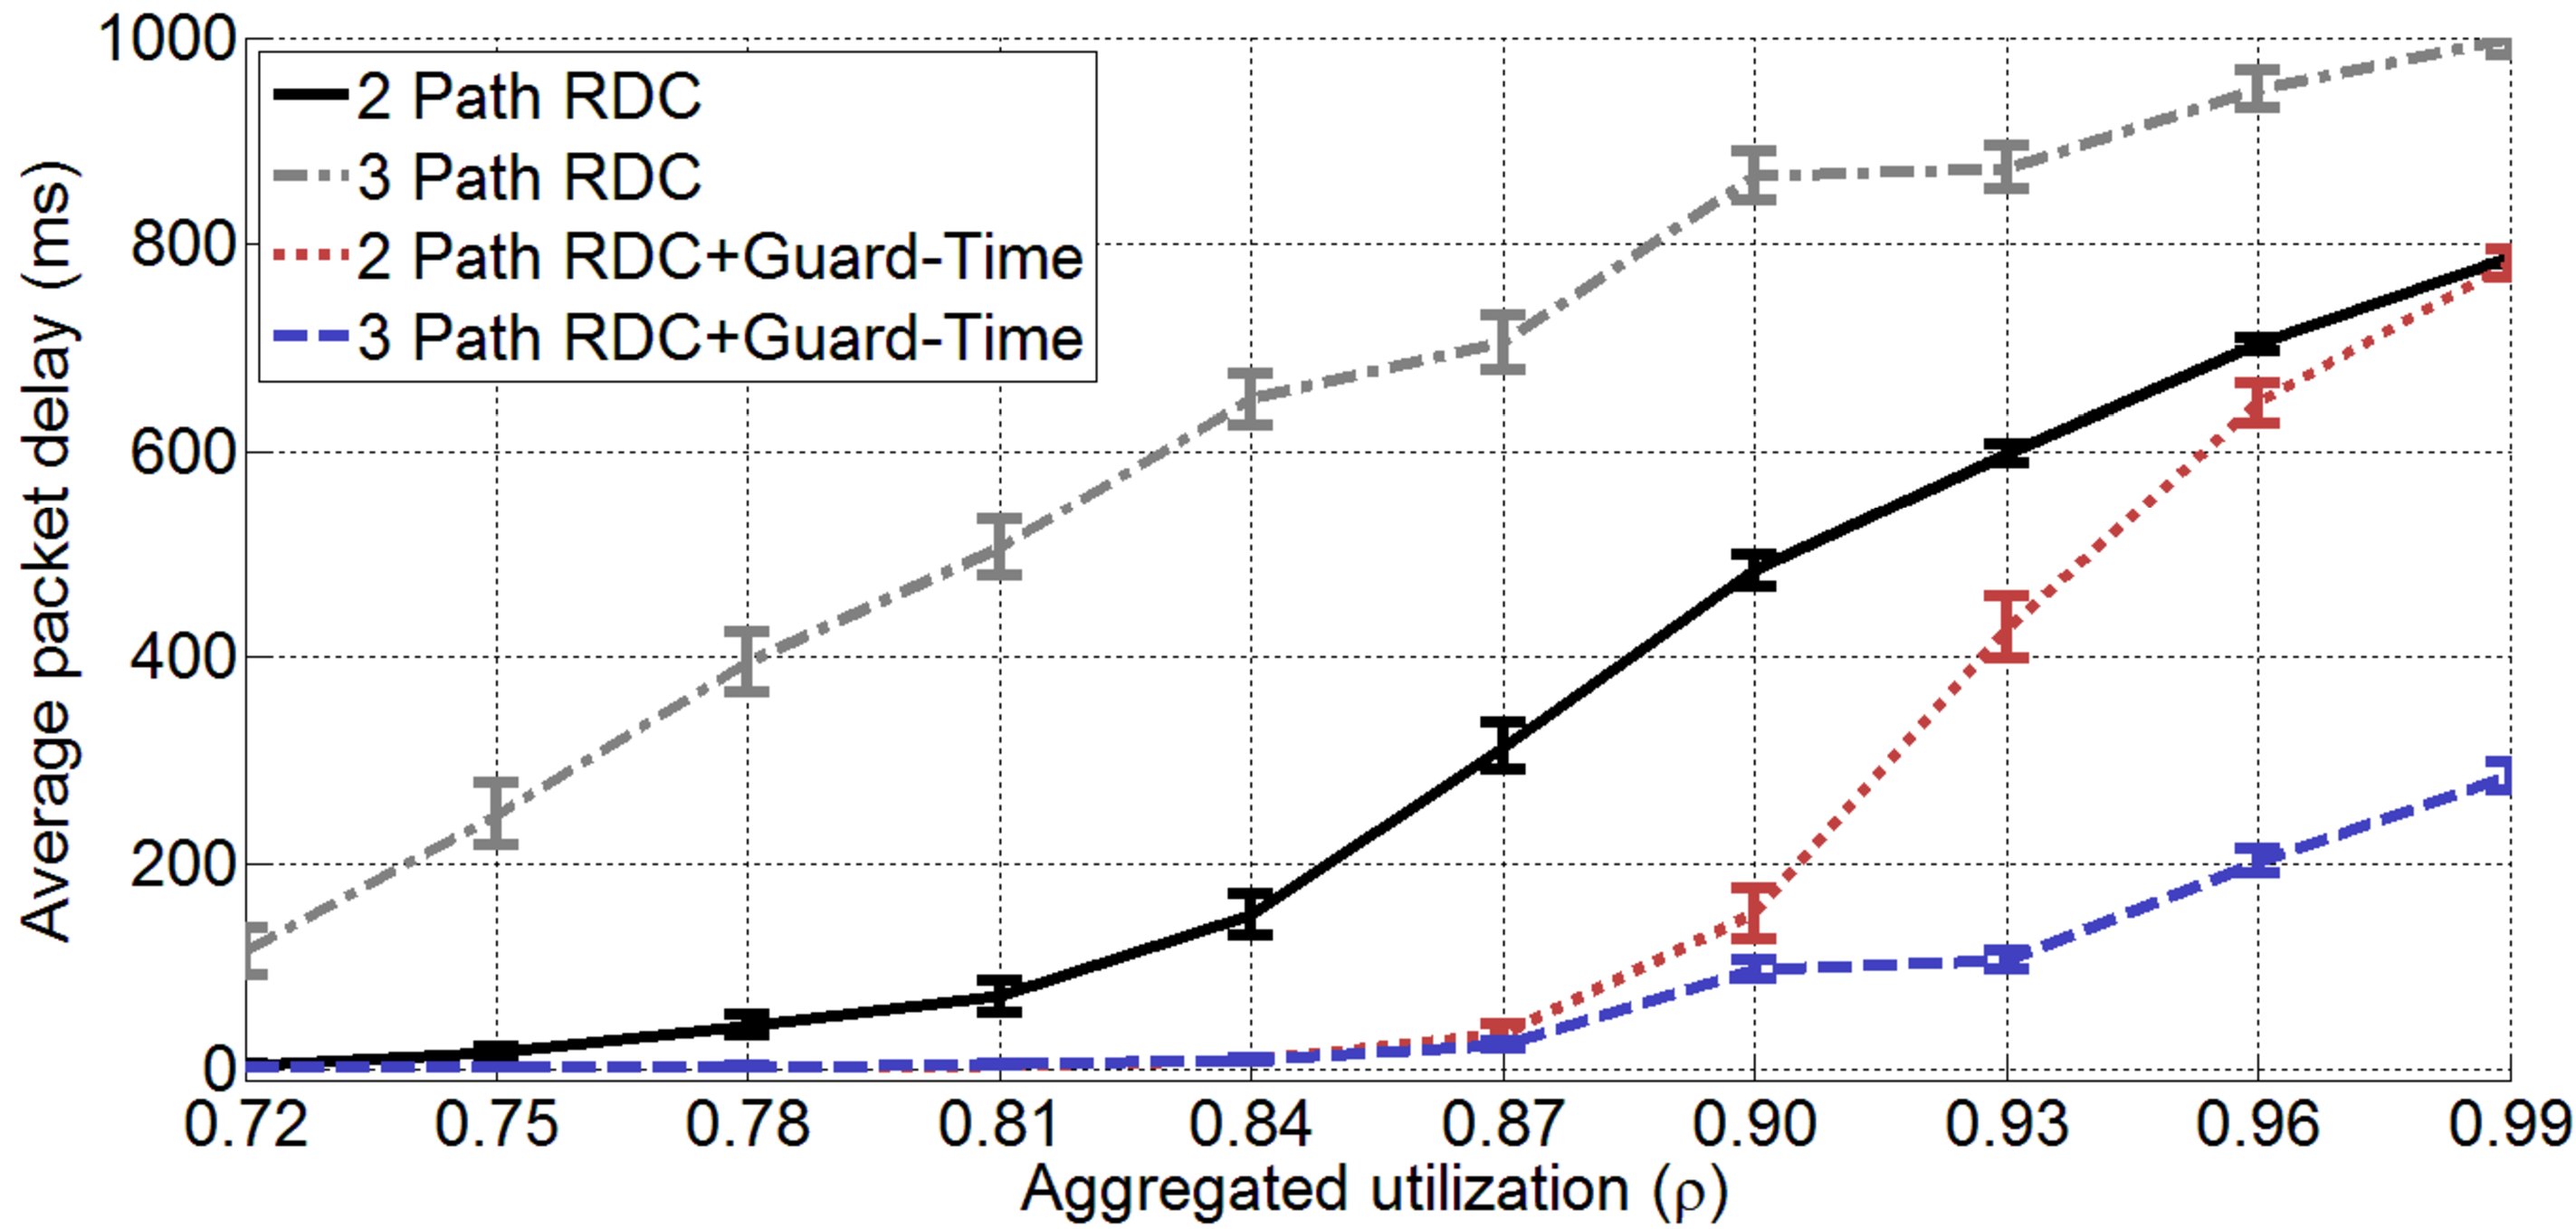
\includegraphics[width=8.8cm,height=4.3cm]{figura8}
	\caption{RDC and RDC+Guard-Time with 3 paths.}
	\label{figura8}
\end{figure}

The pure reactive delay-centric was unable to keep low delay for the transmissions. 
Moreover, the instability of this method increased even more with the addition of the third path.
Unlike the pure RDC, the RDC with guard-time had a better result with the three paths, promoting good distribution of the
transmission among the paths.

\begin{figure}[h!]
	\centering
	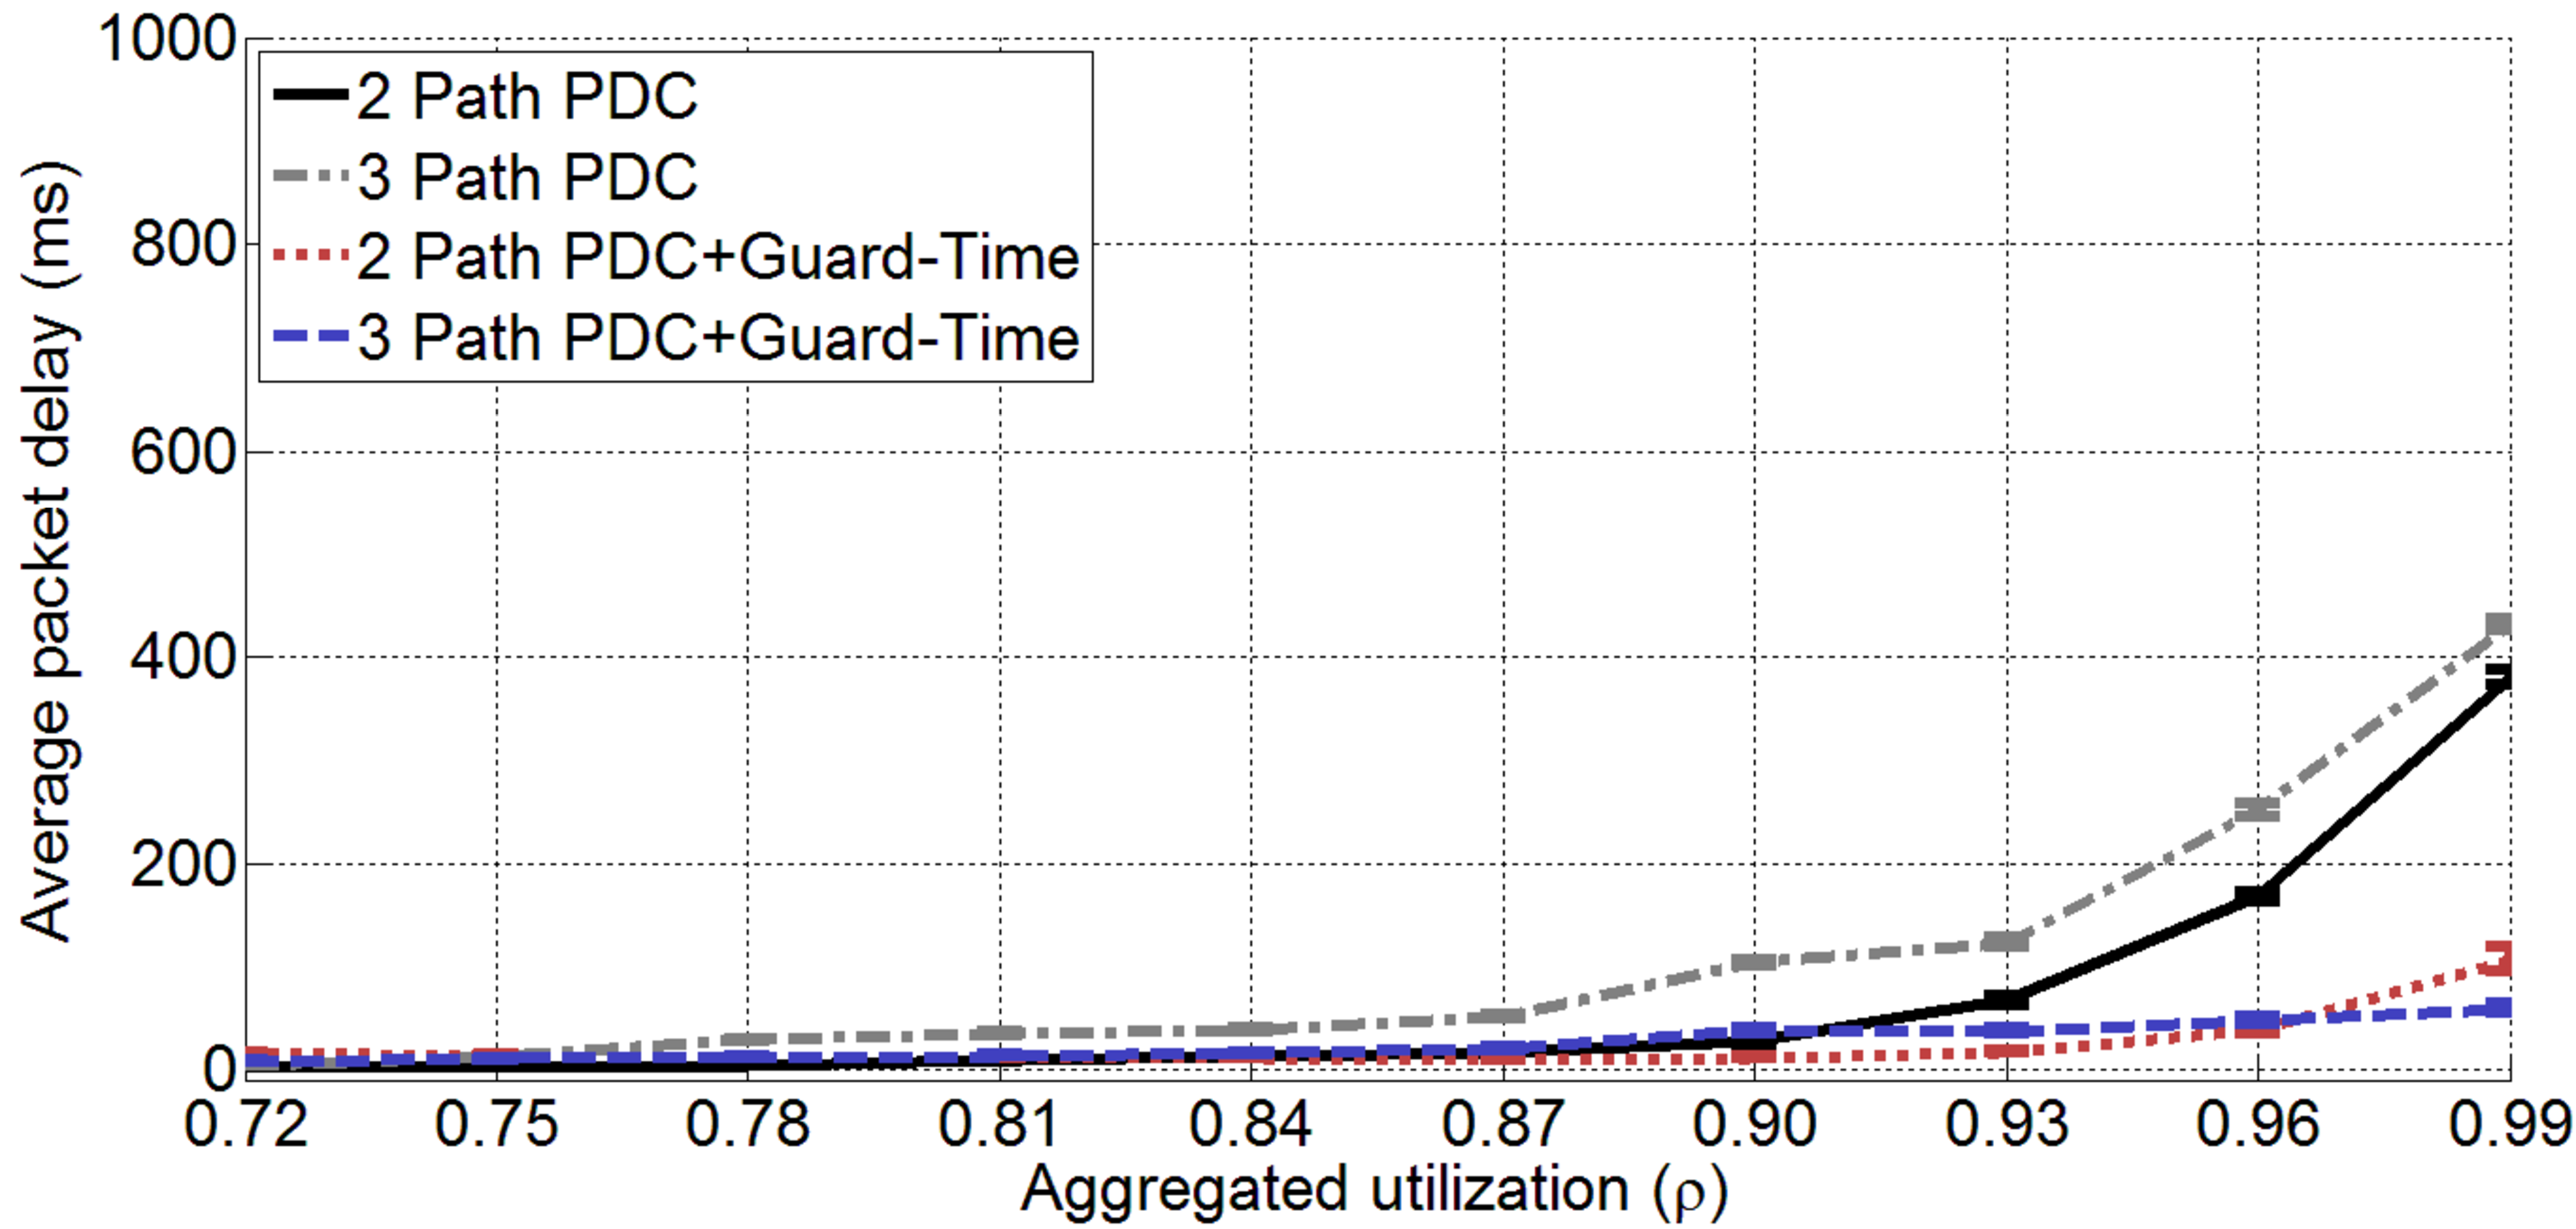
\includegraphics[width=8.8cm,height=4.3cm]{figura9}
	\caption{PDC and PDC+Guard-Time with 3 paths.}
	\label{figura9}
\end{figure}

In Figure~\ref{figura9}, it is possible to see that the differences in the pure PDC method were more discrete, but the addition of the third path also raised the mean delay. The PDC with no guard-time displayed similar result for two and three paths, with low mean delay even for high utilization. 
The only notable difference was for $\rho = 0.99$. In that case, the third path enabled better performance of the method resulting in lower mean delay.


\section{Conclusion}

Low-delay communication is a desired condition for multimedia transmission, such as VoIP calls and video streaming, especially in real-time scenarios. Although delay-centric mechanism for multihomed communication has been efficient to reduce packet delay by selecting the path with smaller SRTT, some instabilities may occur during high utilization when many sources use the same mechanism. This could be a serious problem if the mechanism becomes standard in any multihomed protocol. We confirmed the existence of such instabilities in transmission between two computers with two and three interface cards.

One cause of instability is the poor sampling of the delay in the alternate path. Modification of delay-centric with the introduction of a guard-time and frequent updates of the SRTT in the alternate path significantly reduced these instabilities and consequently the overall mean of the packet delay.

The predictive delay-centric, using trend comparison of current and alternate path also proved to be efficient in reducing the instabilities. The PDC with HB interval reduction during guard-time was able to eliminate almost every instability in the handover mechanism. 

Scenarios with background traffic and the addition of a third path were also investigated. The PDC method with guard-time performed better in all cases as well. Transmissions could be performed at very high utilization with lower mean delay compared to the other methods.


 %\begin{thebibliography}{2}
  %  \bibitem {Lamport} L. Lamport, \textit{A Document Preparation
  %  System: \LaTeX, User's Guide and Reference Manual}. Addison
  %  Wesley Publishing Company, 1986.
  %  \bibitem {Shell} M. Shell, ``How to use the IEEETran \LaTeX class'',
  % \textit{Journal of \LaTeX class files}, vol. 1, no. 8, pp.
  %  1-22. August 2002.
  %\end{thebibliography}

\bibliographystyle{IEEEtran}
\bibliography{referencias}

\end{document}
